\begin{frame}\frametitle{\vspace*{0.5cm}We simulated and US-pulse impinging on a water-air interface}
  \begin{minipage}{0.62\textwidth}
    \begin{minipage}{\textwidth}
      \begin{figure}
        \centering
        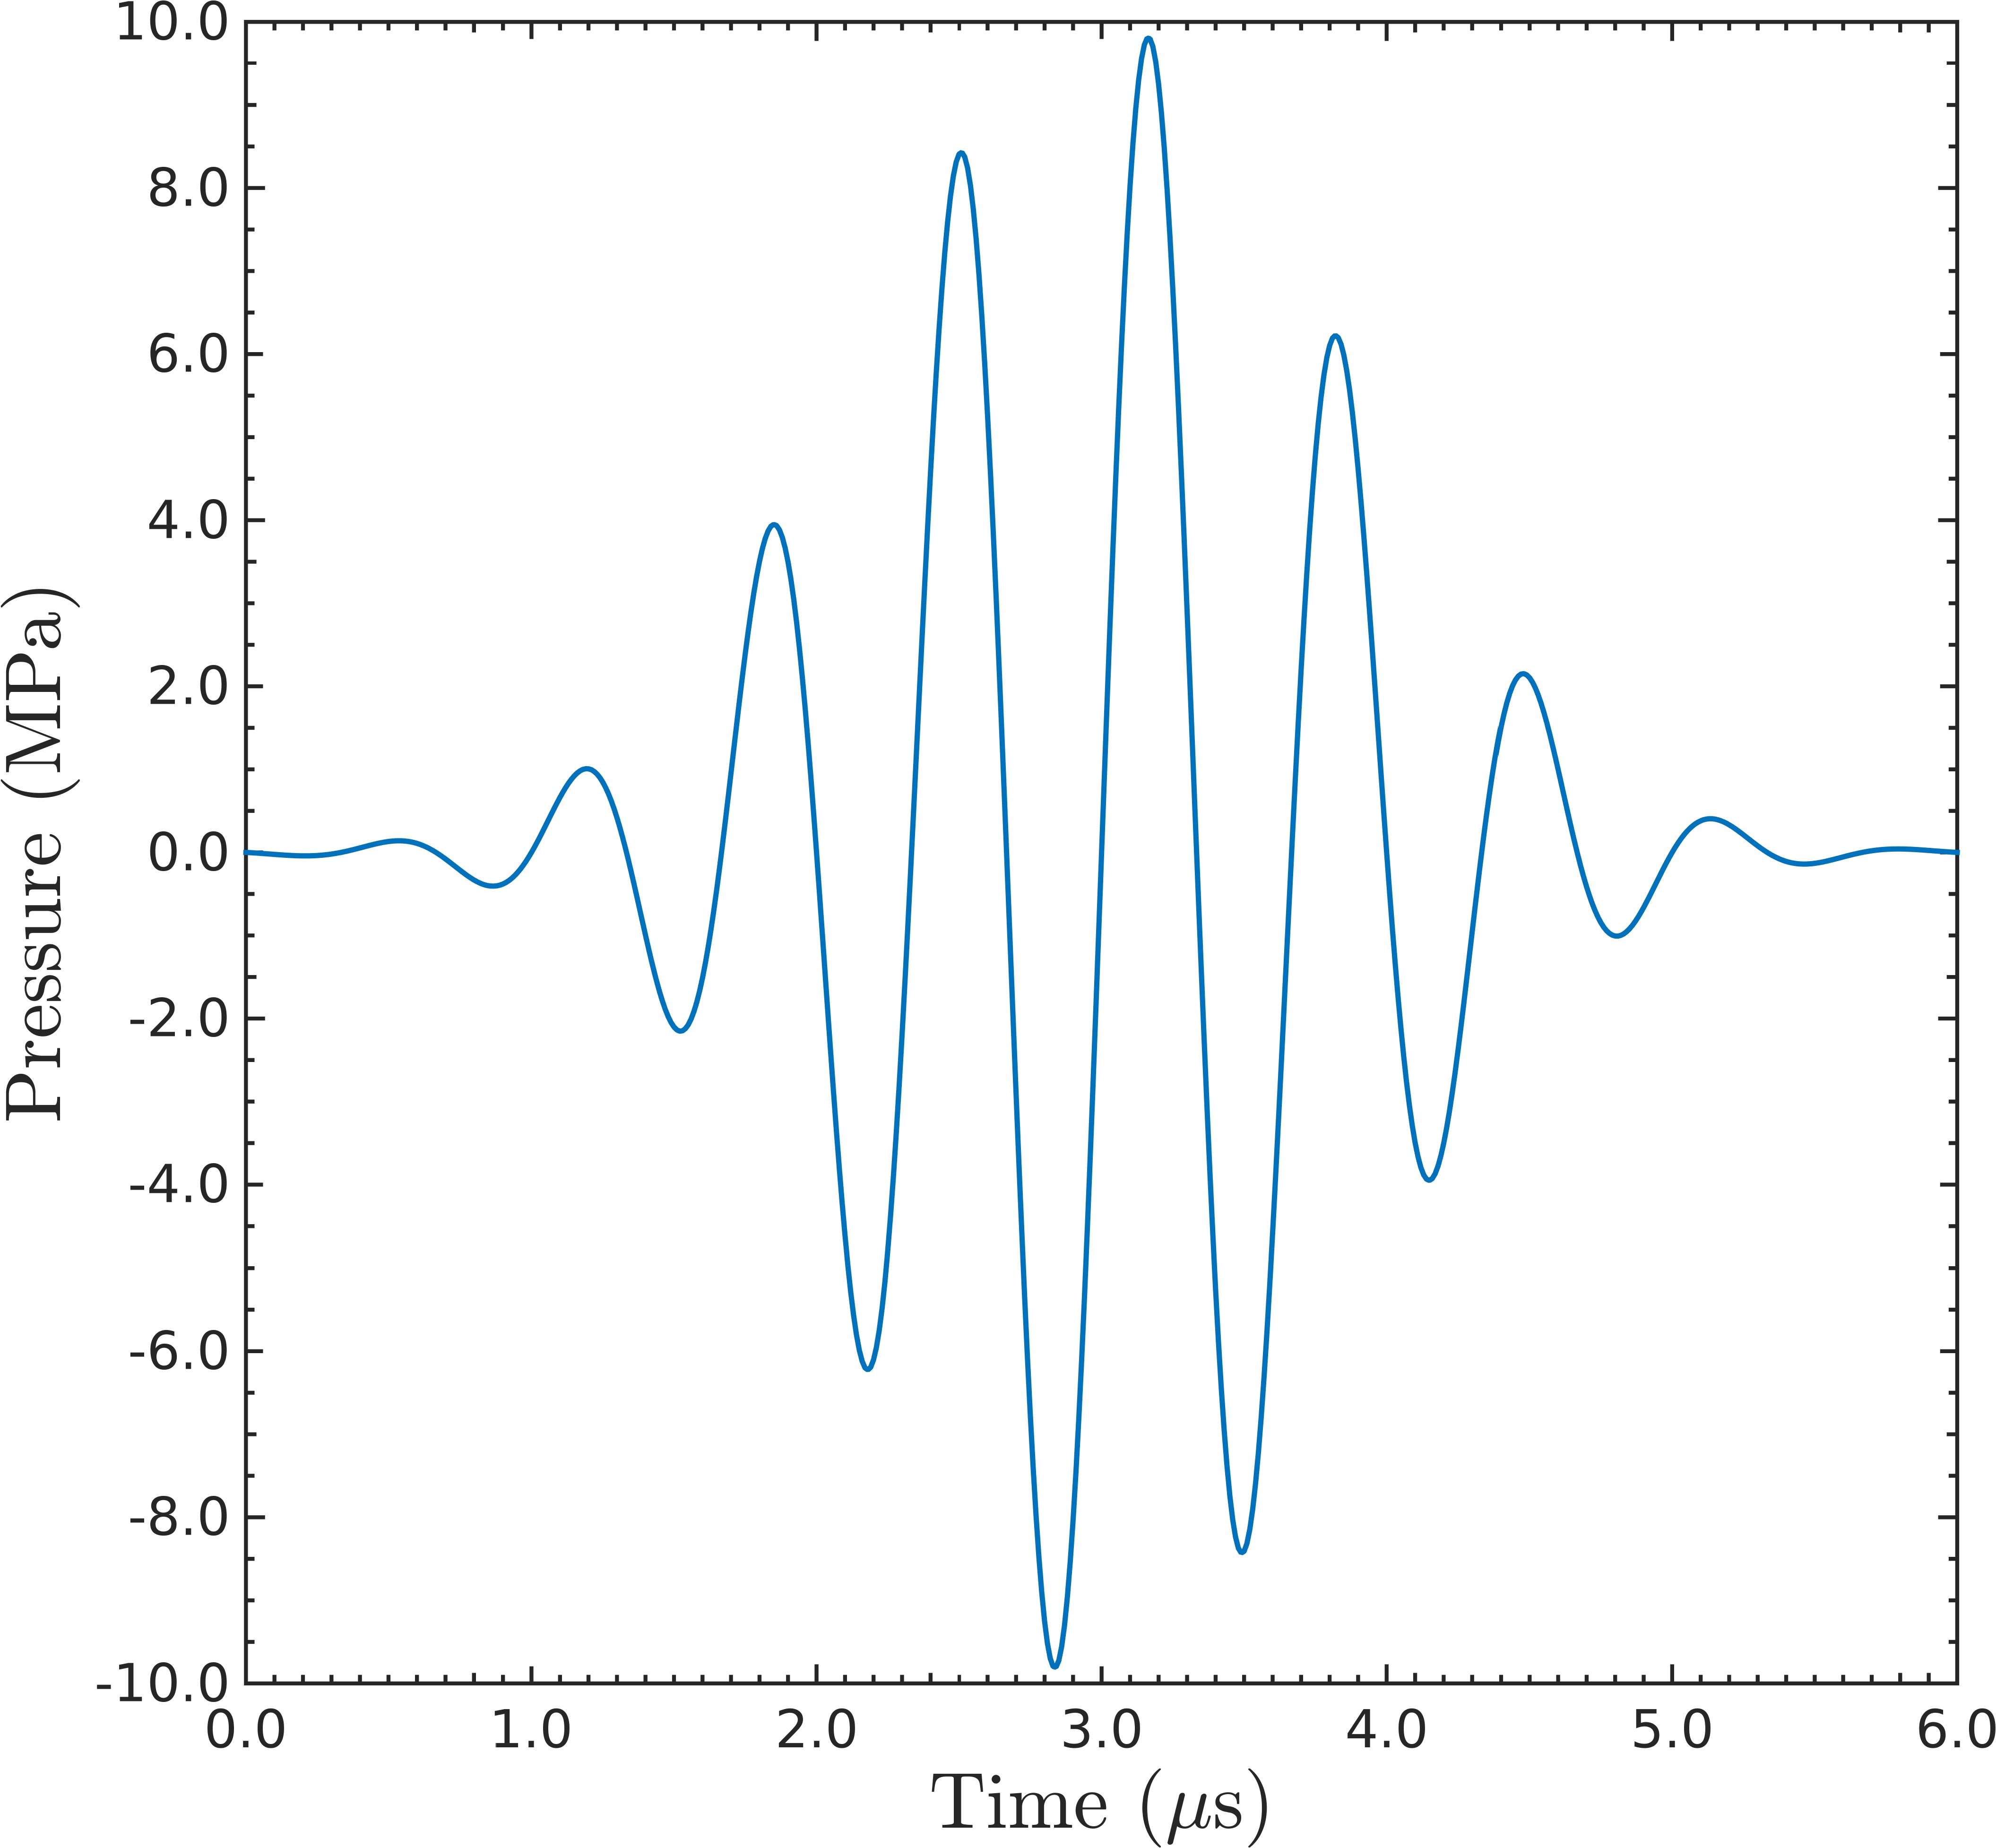
\includegraphics[width=0.47\textwidth]{../figs/lung_figs/p0_vs_t_us}%
         \def\svgwidth{0.48\textwidth} {\footnotesize
           \import{../figs/lung_figs/}{Alveolus_US_zoom_only_diagram.pdf_tex}
          %\import{../figs/lung_figs/}{usbe_lung_schematic3.pdf_tex}
          \hfill%
        }%
      \end{figure}
    \end{minipage}
  % 
%     \begin{minipage}{\textwidth}
%       \begin{figure}
%         \centering \def\svgwidth{0.48\textwidth} {\footnotesize
%           \import{../figs/lung_figs/}{usbe_lung_schematic3.pdf_tex}
%           \hfill%
%         }
% %        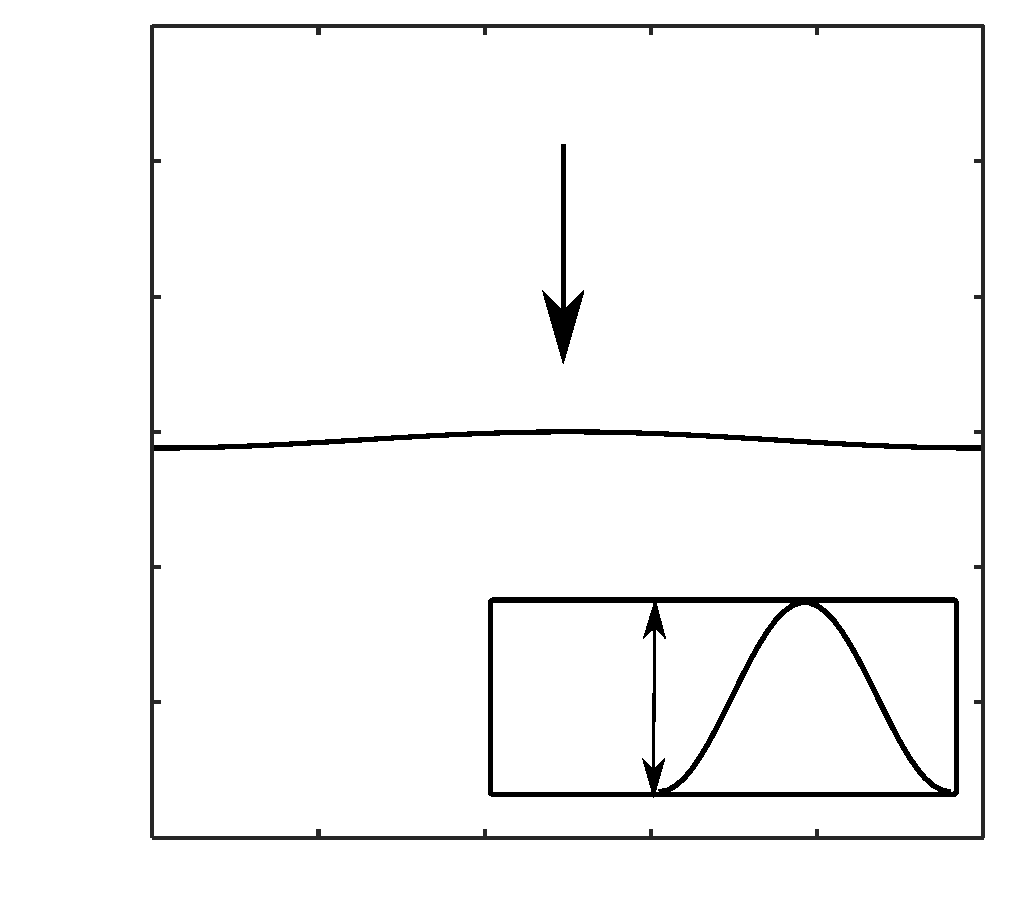
\includegraphics[width=0.48\textwidth]{../figs/lung_figs/usbe_model_schematic}
%       \end{figure}
%     \end{minipage}
  \end{minipage}
  % 
  \hfill
  %
  \begin{minipage}{0.36\textwidth}
    \movie[externalviewer]{%
      \begin{tikzpicture}
          \node[anchor=south west,inner sep=0] (image) at (0,0) {
            \adjincludegraphics[trim={{0.32\width} 0 {0.32\width} 0 },clip=true,height = 0.7\textheight]{./figs/still.jpg}%x
          };%
          \begin{scope}[x={(image.south east)},y={(image.north west)}]%
            \node[font=\tiny,right] at (0.20,0.8) {Water};%
            \node[font=\tiny,right] at (0.20,0.4) {Air};%
            \node[font=\tiny,right] at (0.55,0.85) {Wave};%
            \draw[thick,->] (0.66,0.83) -- (0.66,0.75);%
          \end{scope}%  
        \end{tikzpicture}%
      }%
    {./figs/rmawave_1_10000000.0_0.03_45.0_0.0_1.0_1.0_100_100_blue.avi}
  \end{minipage}
  \vspace*{0.5cm}
  \begin{center}
    \visible<2>{
      \begin{itemize}
      \item Linear acoustics doesn't explain the interface deformation.
      \item The DUS pulse is complicated and not ideal for analysis.
      \end{itemize}
    }
  \end{center}
  %
  \note{
    \begin{enumerate}
    \item So I'll get into the details later, but I want to show a
      preliminary simulation we did of a $10$ MPa US-pulse like waveform
      composed of a sinusoid wrapped in gaussian firing downward from
      water into air.
    \item I'll note that $10$ MPa is high for DUS, but qualitatively similar results were achieved for lower amplitudes, they just moved to slowly for practical computational purposes.
    \item A basic model simulation of this (reference middle figure).
    \item Show video (stop at $10$s if possible).
    \item What I want you to see here is that the interface deforms, in a way that linear acoustics would not predict. That would just predict a vibrating interface.
    \item Also, this DUS pulse is mathematically complicated and not ideal for analysis.
    \end{enumerate}
  }
\end{frame}

%%% Local Variables:
%%% mode: latex
%%% TeX-master: "../main"
%%% End:
